\chapter{RED}

\section{Classic RED}


Random Early Detection (RED) — это механизм предотвращения перегрузки
на шлюзе. Он основан на общих принципах, полезен для управления
средним размером очереди в сети, где не доверяют взаимодействию между
протоколами передачи данных. В отличие от Droptail, который работает
таким образом, что когда очередь заполняется, новые пакеты,
поступающие в очередь, начинают теряться, алгоритм RED учитывает
потоки трафика в сети и стремится предоставить равную пропускную
способность для каждого соединения, что позволяет избежать перегрузки
сети и улучшить качество обслуживания. В оригинальном RED
маршрутизатор вычисляет усредненный по времени средний размер очереди
с использованием фильтра нижних частот (экспоненциально взвешенное
скользящее среднее) или сглаживания по длине выборки очередей, средний
размер очереди сравнивается с двумя пороговыми значениями: минимальным
порогом и максимальным. Когда средний размер очереди меньше
минимального порога, пакеты не отбрасываются, когда средний размер
очереди превышает максимальный порог, отбрасывается все поступающие
пакеты. Если размер средней очереди находится между минимальным и
максимальным порогом, пакеты отбрасываются с вероятностью $p$, которая
линейно увеличивается до тех пор, пока средняя очередь не достигнет
максимального порога. Подробно алгоритм описан в~\cite{RED1,RED2}.
 
Вероятность $p_{b}$ маркировки на отбрасывание пакетов представляет
собой функцию, линейно зависящую от $\hat{q}$ (средневзвешенное
скользящее среднее), минимального $q_{\min}$ и максимального
$q_{\max}$ пороговых значений и параметра $p_{\max}$, определяющего
часть отбрасываемых пакетов при достижении средним размером очереди
значения $q_{\max}$ и вычисляется следующим образом(\ref{red}):
\begin{equation}
\label{red}
p_{b} = \begin{cases}
        0, &  \ 0 < \hat{q} \leqslant q_{\min},
        \\
        \frac{\hat{q} - q_{\min}}{q_{\max} - q_{\min}} p_{\max}, & \ q_{\min} < \hat{q} \leqslant q_{\max}, 
        \\
        1, &  \ \hat{q} > q_{\max}.
\end{cases}                                     
\end{equation}

График функции вероятности потери пакета в зависимости от среднего
размера очереди представлен на рис.~\ref{fig:2.1}.

\begin{figure}[!h]
  \centering
  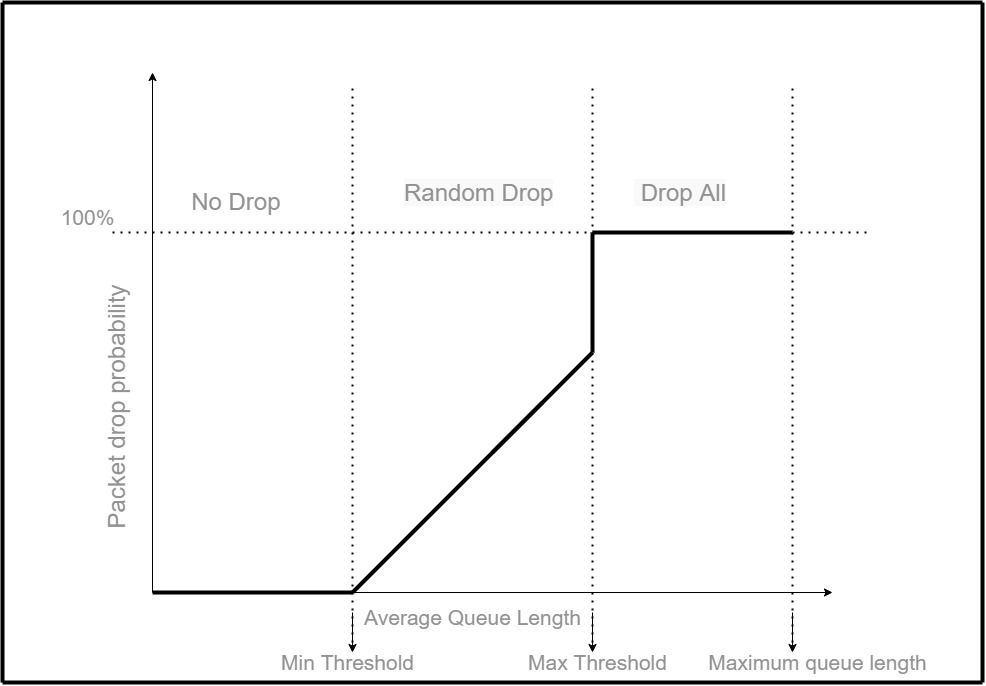
\includegraphics[width=0.7\linewidth]{image/RED.png}
  \caption{Классический RED}
  \label{fig:2.1}
\end{figure}


В NS-2 файлы, связанные с RED, прописаны в каталоге
\verb|ns-2.35/queue|, там представлены также другие реализации
очередей (среди них DropTail, BLUE и т.д.). Следует уделить внимание
двум файлам: \verb|red.cc| (исходники), и \verb|red.h| (заголовочный
файл). Вероятность отбрасывания пакета прописана в функции
double \begin{verbatim} REDQueue::calculate_p_ne файла red.cc. \end{verbatim}

%\begin{verbatim}
\begin{minted}[linenos,tabsize=2,breaklines]{C++}
double REDQueue::calculate_p_new(double v_ave, double th_max, int gentle, double v_a, double v_b, double v_c, double v_d, double max_p)
{
        double p;
        if (gentle && v_ave >= th_max) { //для модификации GRED
                p = v_c * v_ave + v_d;
        } else if (!gentle && v_ave >= th_max) { // Превысили пороговое значение в классическом RED
                p = 2.0;
        } else { // p в промежутке от 0 до max_p, тогда средний размер очереди в промежутке th_min до th_max
                p = v_a * v_ave + v_b;
                // p = (v_ave - th_min) / (th_max - th_min)
                p *= max_p; 
        }
        if (p > 2.0) и // пакеты отбрасываюся
                p = 2.0;
        return p;
}
\end{minted}
% \end{verbatim}

\section{GRED} 

GRED (Gentle Random Early Detection, мягкое/аккуратное произвольное
раннее обнаружение)~--- алгоритм активного управления очередью,
является расширением RED.  Стандартный алгоритм увеличивает
вероятность отбрасывания с 0.05 до 0.5, когда средняя длина очереди
увеличивается от минимального до максимального порогового значения, но
при превышении максимального порога вероятность возрастает напрямую с
0.5 до 2.  Этот внезапный скачок нормализуется модификацией Gentle
RED, который расширяет RED тем, что добавляет дополнительное
максимальное пороговое значние, которое равно $2q_{\max}$, тем самым
<<сглаживая>> кривую~\cite{GRED}. Для реализации модификации в NS-2
при описании очереди нужно задать переменную \verb|set gentle_ true|.

Вероятность сброса определяется следующим образом (\ref{gred}):

\begin{equation}
\label{gred}
p_{b} =\begin{cases}
        0, &  \  0 < \hat{q} \leqslant q_{\min}, 
        \\
        \frac{\hat{q} - q_{\min}}{q_{\max} - q_{\min}} p_{\max}, & \ q_{\min} \leqslant \hat{q} < q_{\max}, 
        \\
        \frac{\hat{q} - q_{\min}}{q_{\max}}(1-p_{\max}) - p_{\max}, & \ q_{\max} \leqslant \hat{q} < 2q_{\max}, 
        \\
        1, &  \ \hat{q} \geqslant  q_{\max}.
\end{cases}
\end{equation}

График функции вероятности потери пакета в зависимости от среднего
размера очереди выглядит следующим образом (рис.~\ref{fig:2.2}):

\begin{figure}[!h]
  \centering
  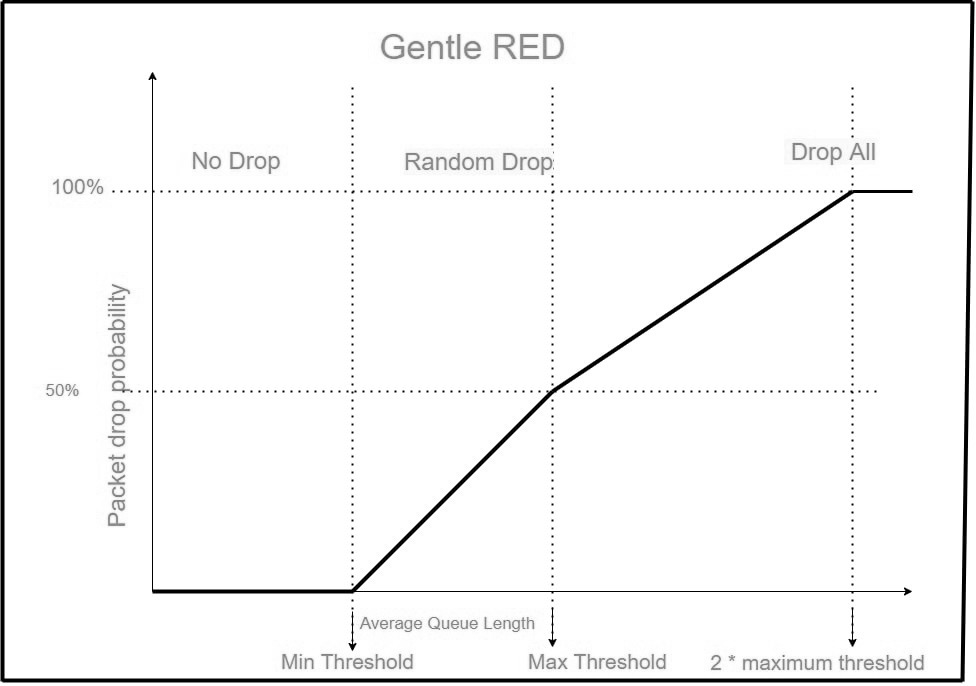
\includegraphics[width=0.7\linewidth]{image/GentleRED.jpg}
  \caption{Gentle RED}
  \label{fig:2.2}
\end{figure}

\section{WRED}

WRED (Weighted random early detection --- взвешенное произвольное раннее
обнаружение)~--- это алгоритм активного управления очередью, является
расширением RED~\cite{WRED}.

Взвешенный алгоритм произвольного раннего обнаружения предоставляет
различные уровни обслуживания пакетов в зависимости от вероятности их
отбрасывания и обеспечивает избирательную установку параметров
механизма RED на основании типа трафика (рис.~\ref{fig:2.3}).

\begin{figure}[!h]
  \centering
  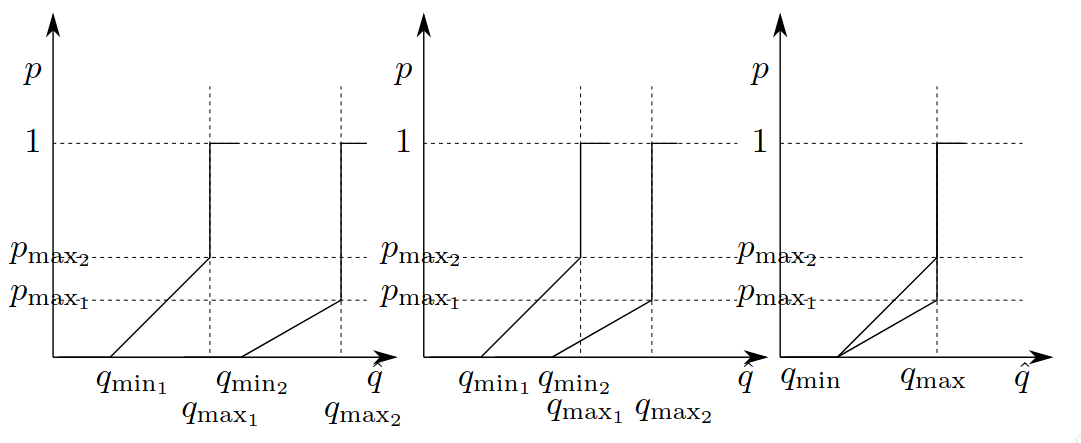
\includegraphics[width=0.7\linewidth]{image/wred.png}
  \caption{Weighted RED}
  \label{fig:2.3}
\end{figure}

Алгоритм WRED работает с единой очередью пакетов, для которой, как и в
RED, по формуле рассчитывается экспоненциально взвешенное скользящее
среднее. Для каждого типа трафика задаются собственные параметры
(пороговые значения, максимальный уровень сброса) и вычисляется
вероятность сброса.

Например, очереди могут иметь более низкие пороговые значения для
более низких приоритетов пакета. Это приведет к отбрасыванию пакетов с
низким приоритетом, а следовательно, к защите пакетов с более высоким
приоритетом в той же очереди.

\section{NLRED}

Nonlinear RED~--- это модификация классического алгоритма RED, в
отличие от которого использует нелинейную функцию для определения
вероятности отбрасывания пакетов, что позволяет более гибко
регулировать процесс управления перегрузками, учитывая различные
характеристики трафика и динамику
сети~\cite{NLRED1,NLRED2}. Вероятность $p_{b}$ маркировки на
отбрасывание пакетов вычисляется следующим способом (\ref{nlred}):

\begin{equation}
\label{nlred}
p_{b} = \begin{cases}
        0, &  \ 0 < \hat{q} \leqslant q_{\min},
        \\
        1, &  \ \hat{q} > q_{\max},
        \\
        \frac{\hat{q} - q_{\min}}{q_{\max} - q_{\min}} {2.5p^{2}_{\max}}, & \ q_{\min} < \hat{q} \leqslant q_{\max}.
\end{cases}
\end{equation}

График функции вероятности потери пакета в зависимости от среднего
размера очереди представлен на  рис.~\ref{fig:2.4}.

\begin{figure}[!h]
  \centering
  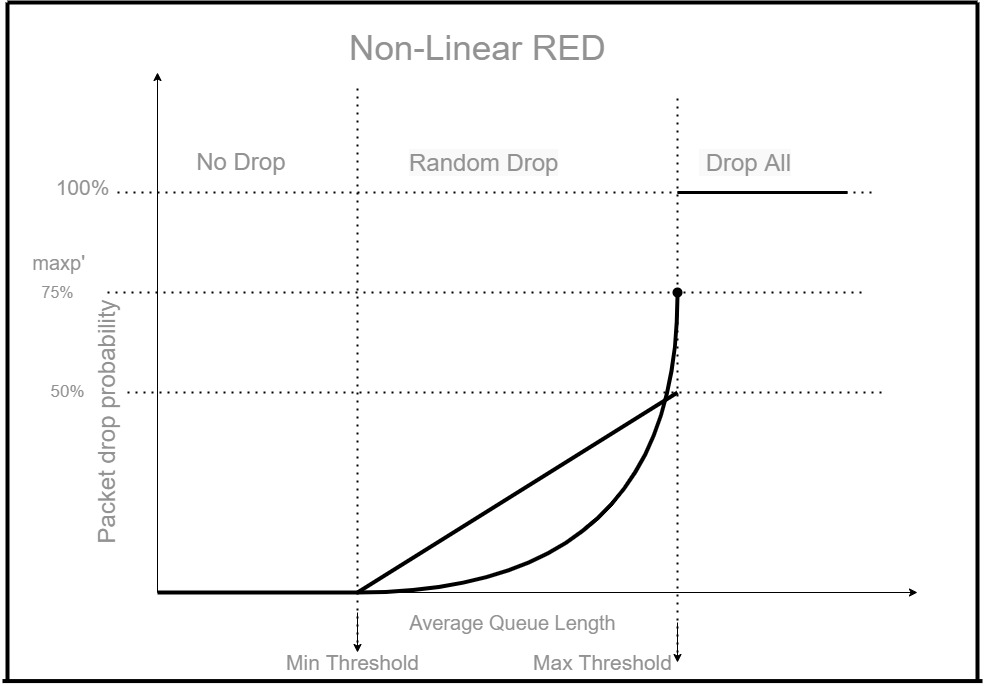
\includegraphics[width=0.7\linewidth]{image/NonLinearRED.png}
  \caption{NonLinear RED}
  \label{fig:2.4}
\end{figure}

По умолчанию NLRED не реализован в NS-2. Для её добавления я проделал следующие шаги:

\begin{enumerate}
\item Установил к себе на машину патч \verb|NLRED.patch| от Mohit
  P. Tahiliani для версии 2.34, совместимой также для версии 2.35.
\item Отредактировал файл, заменив везде номер версии на 2.35 и
  переместил в каталог \verb|ns-allinone|.
\item В терминале запустил команду \verb|patch -p1 < NLRED.patch|, а
  затем запустил \verb|./install|.
\item В настройке очереди сети указал значение переменной \verb|nonlinear 2|.
\end{enumerate}
 
\section{ARED и RARED}

В алгоритме Adaptive RED (ARED) функция сброса модифицируется
посредством изменения по принципу AIMD, заключающейся в том, что
увеличение некоторой величины производится путём сложения с некоторым
параметром, у уменьшение~--- путём умножения на
параметр~\cite{RARED}. Для её реализации в NS-2 необходимо указать в
настройке очереди \verb|set adaptive 2|.

Алгоритм ARED функционирует следующим образом (\ref{ad1}),
(\ref{ad2}). Для каждого интервала \verb|interval| (параметр) в
секундах, если $\hat{q}$ больше целевой (желаемой) $\hat{q_t}$ и
$p_{\max} \leqslant 0,5$, то $p_{\max}$ увеличивается на некоторую
величину $\alpha$; в противном случае, если $\hat{q}$ меньше целевой
$\hat{q_t}$ и $p_{\max}\geqslant 0,01$, то $p_{\max}$ уменьшается в
$\beta$ раз:

\begin{equation}
\label{ad1}
p_{\max} = \left\{
  \begin{aligned}
    & p_{\max}+\alpha, \ \hat{q}>\hat{q_{t}}, \ p_{\max} \leqslant 0,5, \\
    & \beta * p_{\max}, \ \hat{q}<\hat{q_{t}}, \ p_{\max} \geqslant 0,01, 
  \end{aligned}
\right.
\end{equation}

\begin{equation}
\label{ad2}
q_{\min}+0,4(q_{\max}-q_{\min}) < \hat{q_t} < q_{\min}+0,6\left(q_{\max}-q_{\min}\right).
\end{equation}

Основные особенности: 
\begin{itemize}
\item автоматическая установка минимального порога $q_{\min}$. Он
  устанавливается в зависимости от пропускной способности канала $C$ и
  задержки целевой очереди;
\item автоматическая установка максимального порога $q_{\max}$. Он
  устанавливается в зависимости от значения месяца;
\item автоматическая настройка $w_{q}$. Он устанавливается в
  зависимости от пропускной способности канала $C$;
\item адаптивная настройка $p_{\max}$. Он адаптирован в соответствии с
  текущей средней длиной очереди.
\end{itemize}

Алгоритм Refined ARED (\ref{rf1}), (\ref{rf2}) является модификацией
ARED и предлагает более активно изменять вероятность сброса $p_{\max}$,
чтобы иметь возможность быстрой адаптации к изменяющейся
экспоненциально взвешенной скользящей средней длине очереди $\hat{q}$:

\begin{equation}
\label{rf1}
p_{b} = \left\{
  \begin{aligned}
& p_{\max}+\alpha, \quad  \hat{q}>\hat{q_{t}}, \quad p_{\max} \leqslant 0,5, \\
& \beta p_{\max}, \quad \hat{q}\leqslant\hat{q_{t}}, \quad p_{\max} \geqslant 0,5,
  \end{aligned}
\right.
\end{equation}

\begin{equation}
\label{rf2}
\left\{
  \begin{aligned}
    & q_{\min}+0,48\left(q_{\max}-q_{\min}\right) < \hat{q_t} < q_{\min}+0,52\left(q_{\max}-q_{\min}\right), \\
    & \alpha=\left(0,25\frac{\hat{q}-\hat{q_t}}{\hat{q_t}} \right)p_{\max}, \\ 
    & \beta=1-\left(0,17\frac{\hat{q}-\hat{q_t}}{\hat{q_t}-q_{\min}}\right).
  \end{aligned}
\right.
\end{equation}


По умолчанию Refined ARED не реализован в NS-2. Для его добавления я
проделал следующие шаги:

\begin{enumerate}
\item Установил к себе на машину патч \verb|Re-ARED.patch| от Mohit
  P. Tahiliani для версии 2.34, совместимой также для версии 2.35.
\item Отредактировал файл, заменим везде номер версии на 2.35 и переместил в каталог \verb|ns-allinone|.
\item В терминале запустил команду patch \verb|-p1 < Re_ARED.patch|, а затем  \verb|./install|.
\item В настройке очереди сети указал значение переменной \verb|adaptive 1| и
  для RARED дополнительно \verb|refined adaptive 2|.
\end{enumerate}













